%\documentclass{article}
%\usepackage{graphicx,subfigure}
%\usepackage{caption,rotating}
%\begin{document}

\begin{figure}[!h]
\centering
\captionsetup{width=0.7\textwidth}
 \subfigure[Sheep 3437 Wrinkled]{
%   \label{fig:trial1he(i)}
%   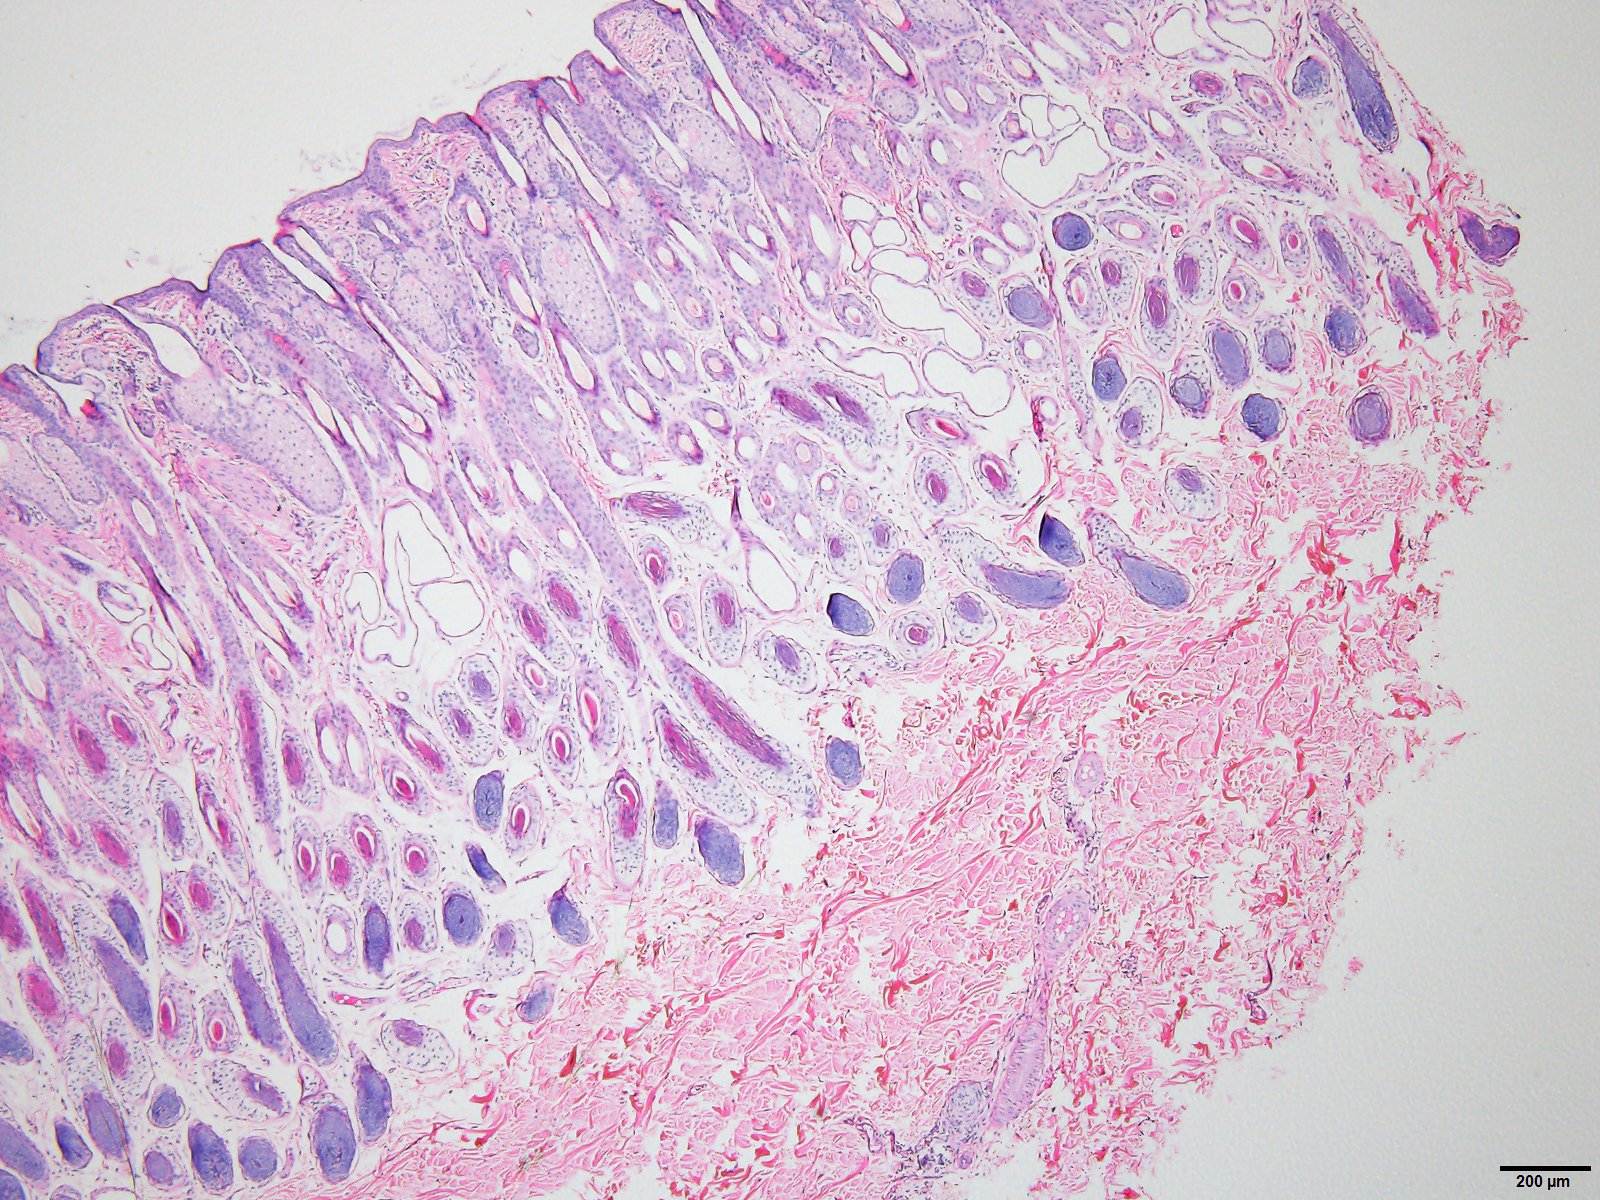
\includegraphics[scale=0.20]{3437_on_wrinkle_4x.jpg}
%    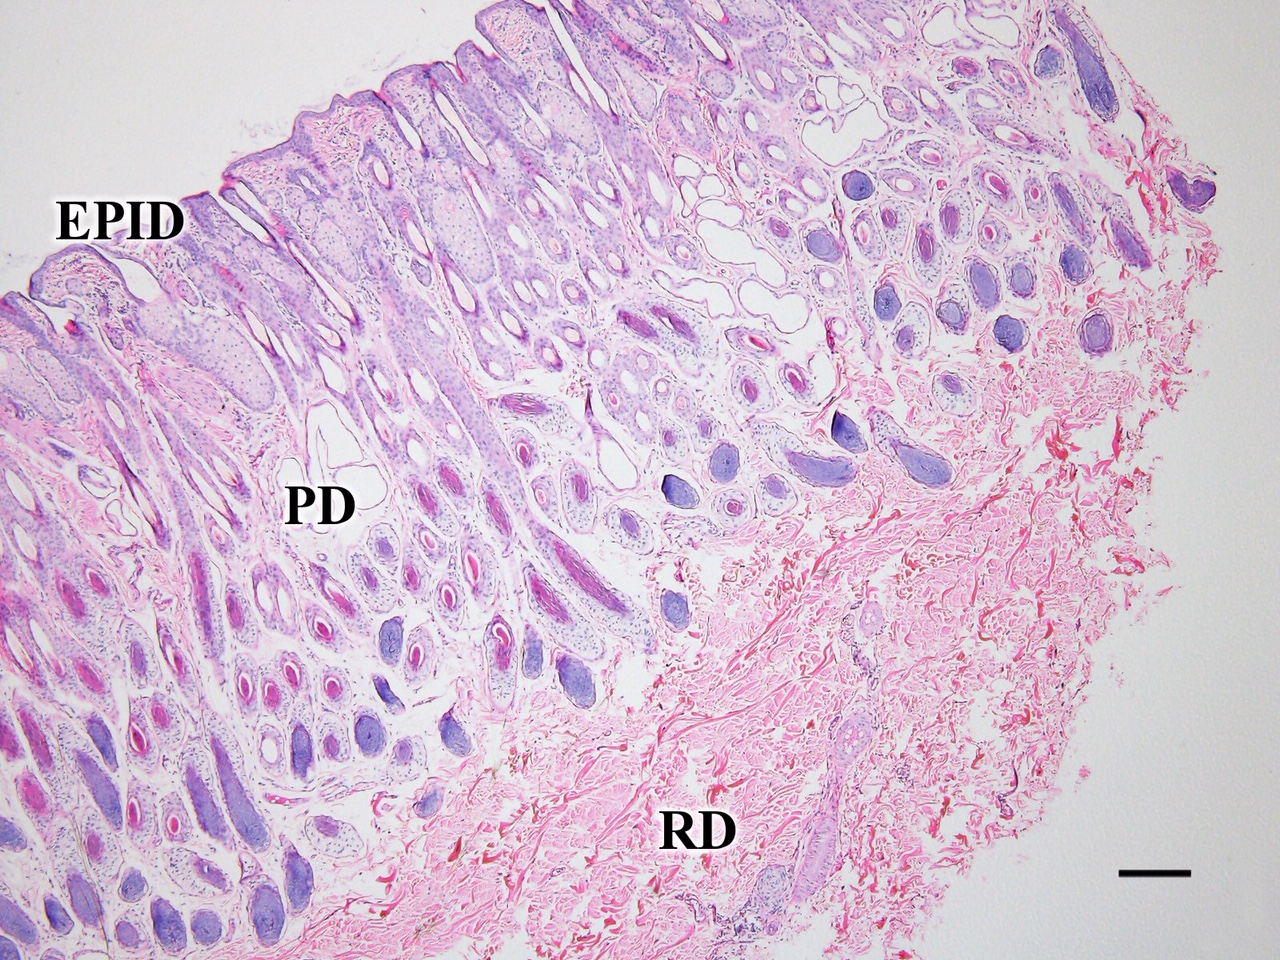
\includegraphics[scale=0.10]{fig2a.jpg}
     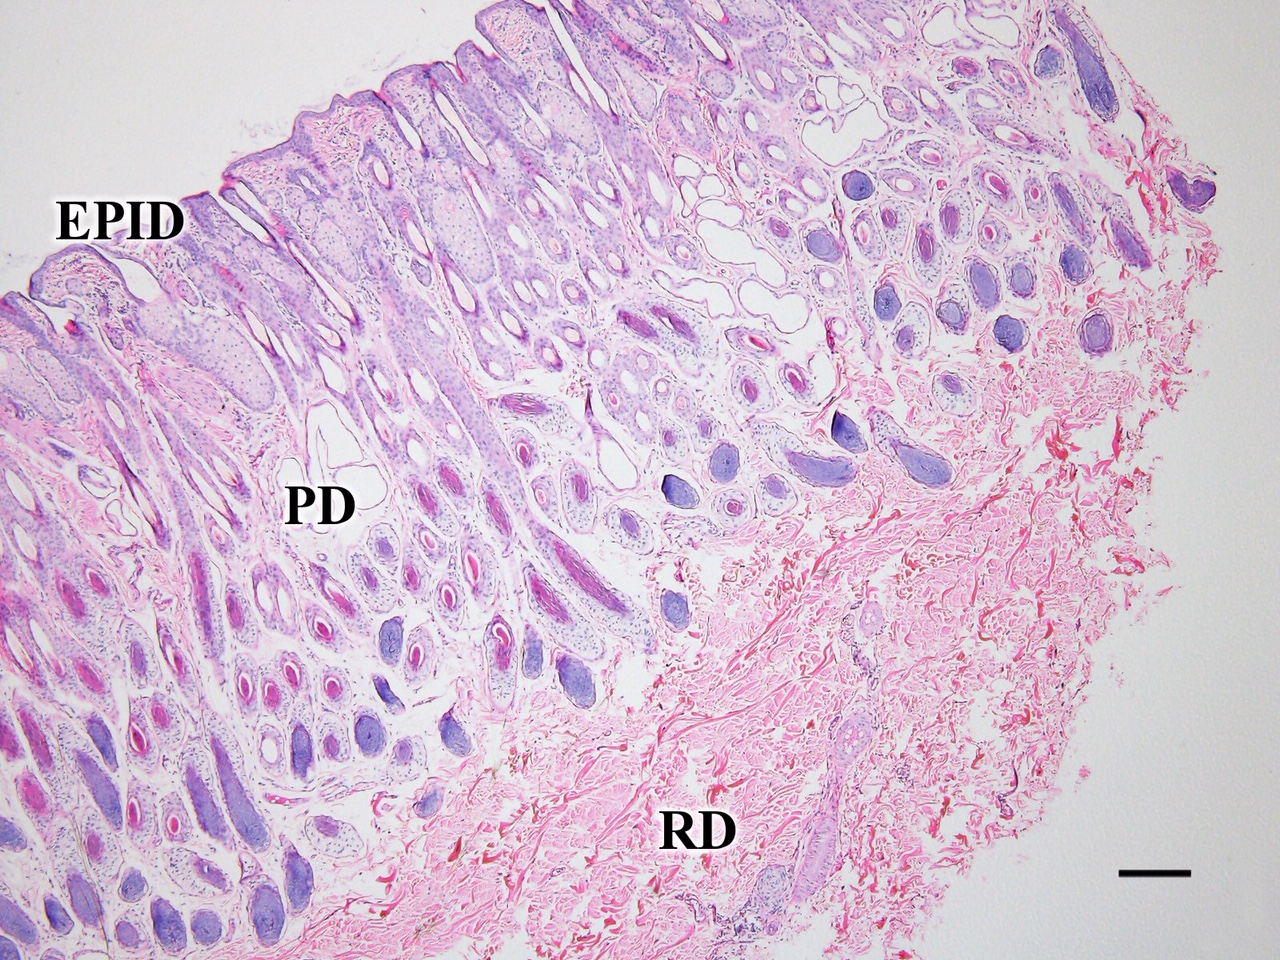
\includegraphics[width=0.7\textwidth]{fig2a.jpg}
% 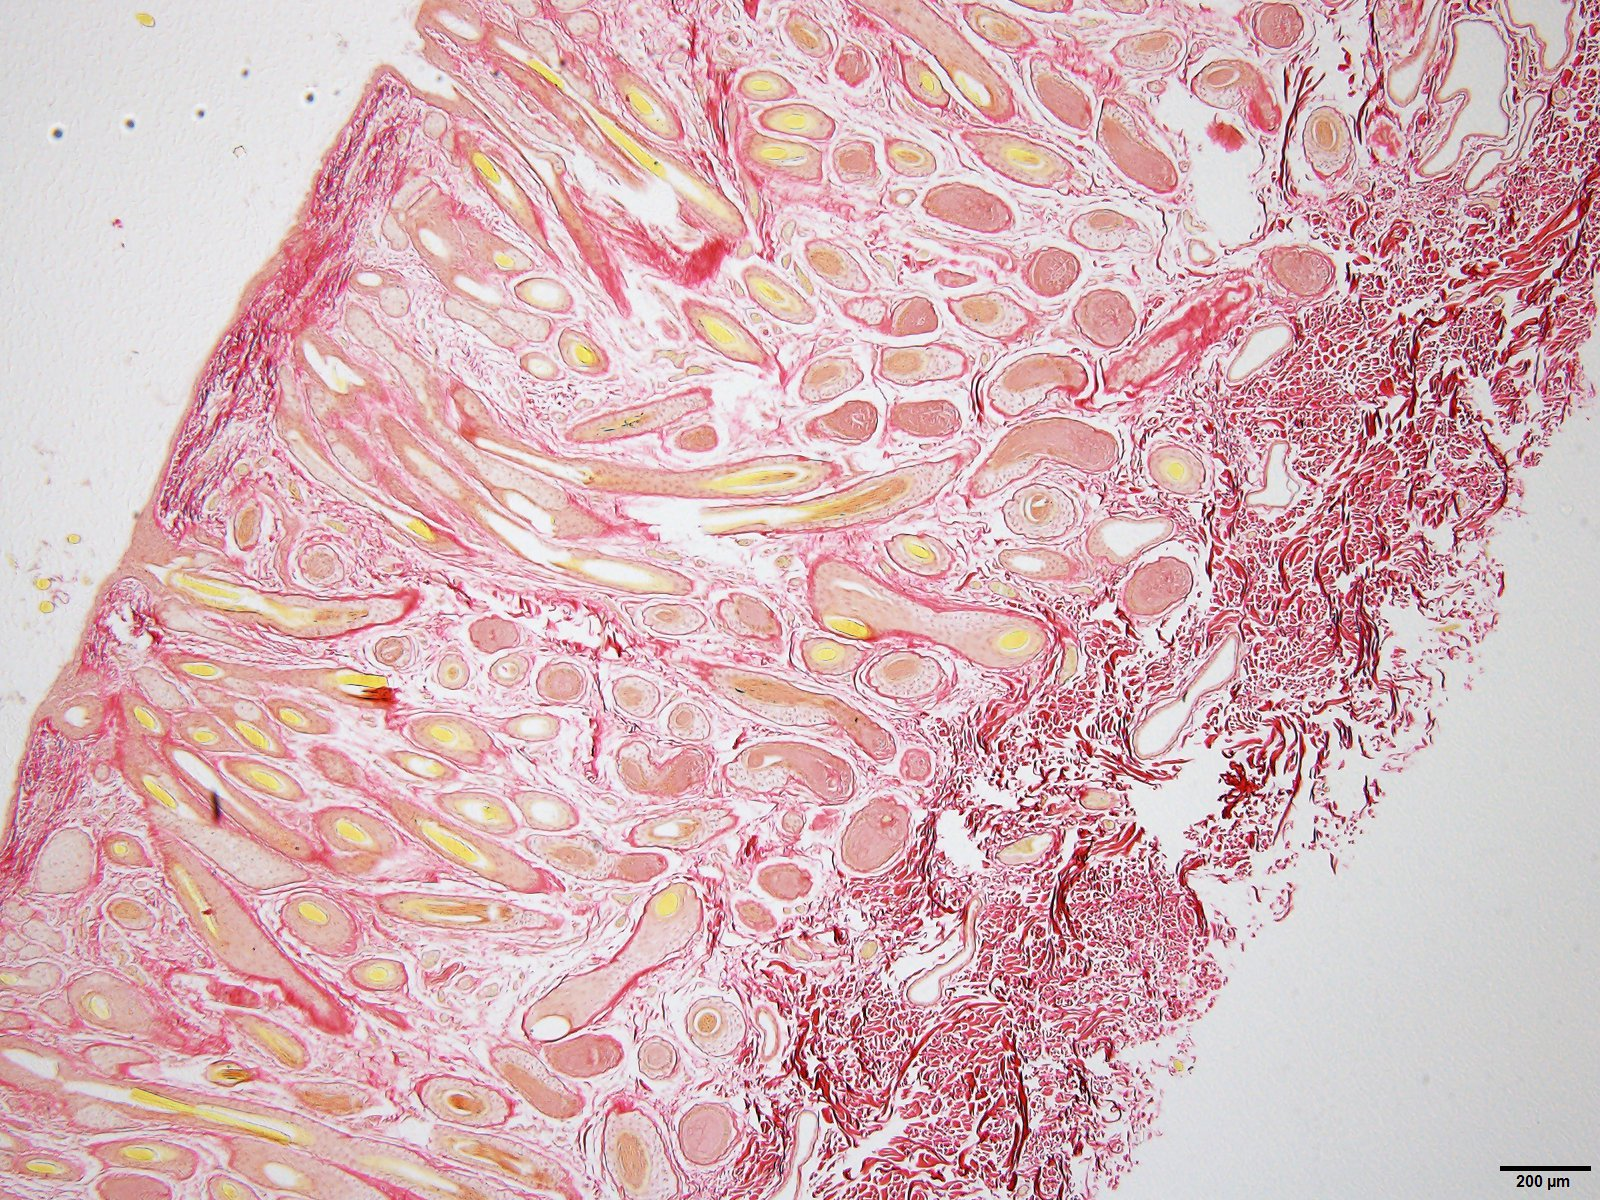
\includegraphics[width=1.0\textwidth]{w479-2-rigid.jpg}
  }
 \subfigure[Sheep 3457 Wrinkle-free]{
%   \label{fig:trial1he(ii)}
%   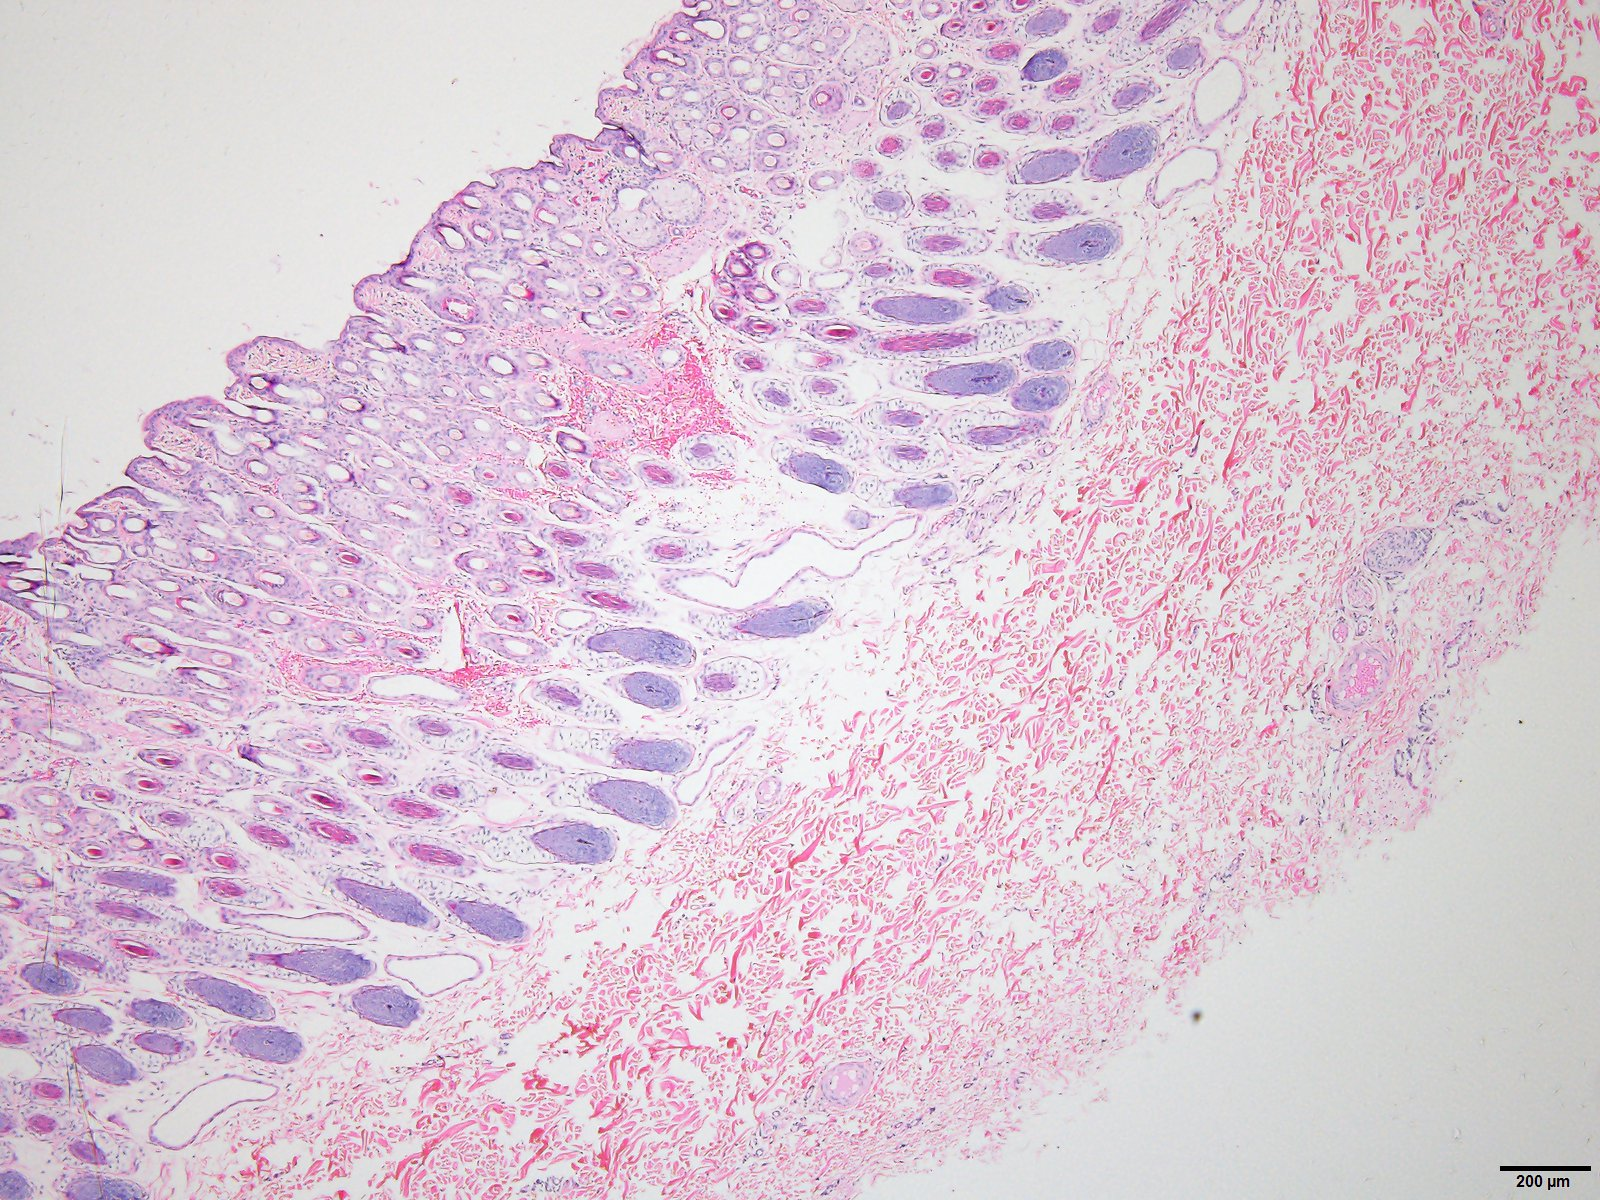
\includegraphics[scale=0.20]{JW_3457_smooth_4x.jpg}
%    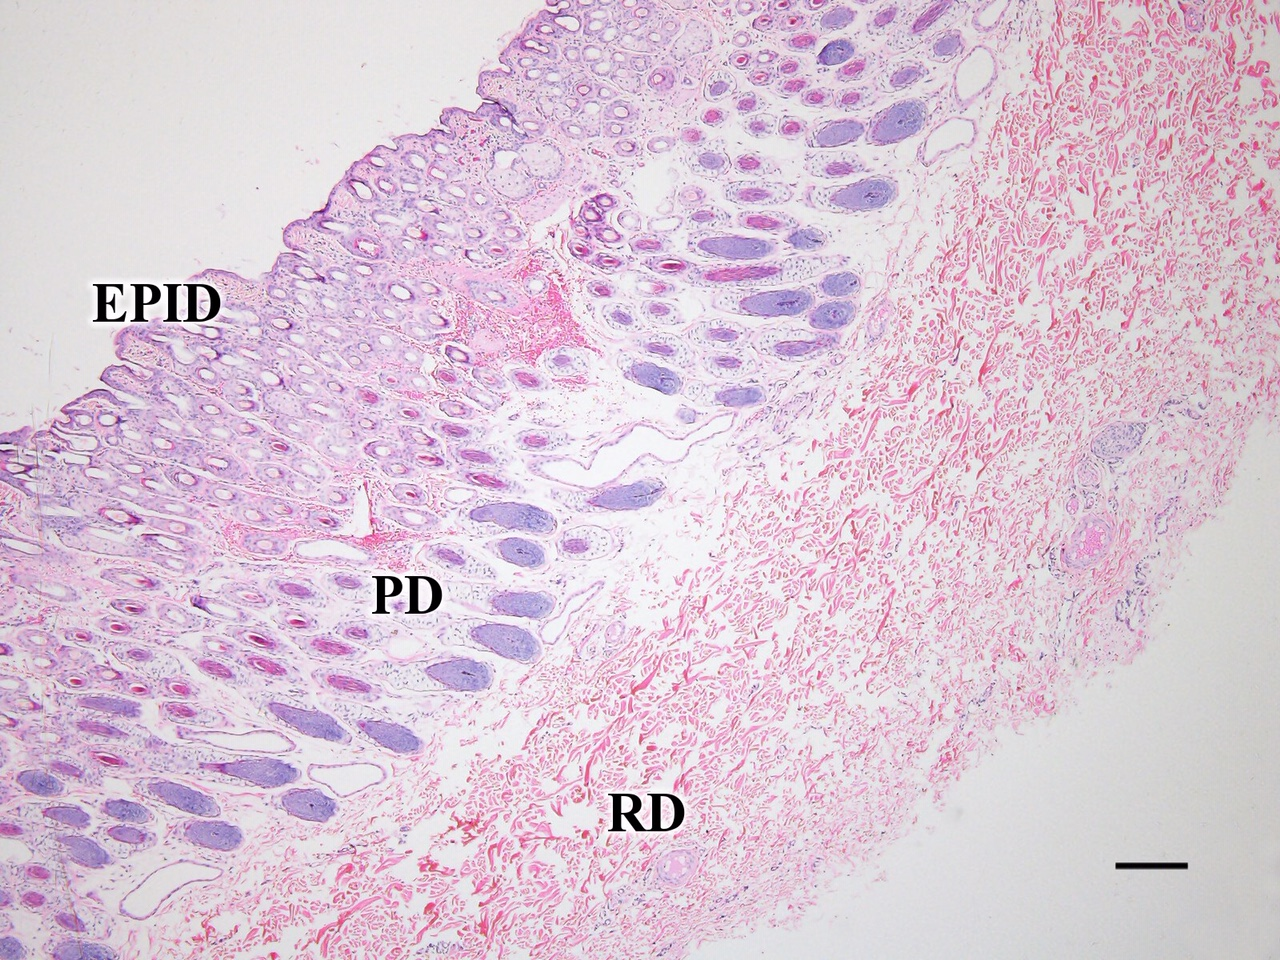
\includegraphics[scale=0.10]{fig2b.jpg}
     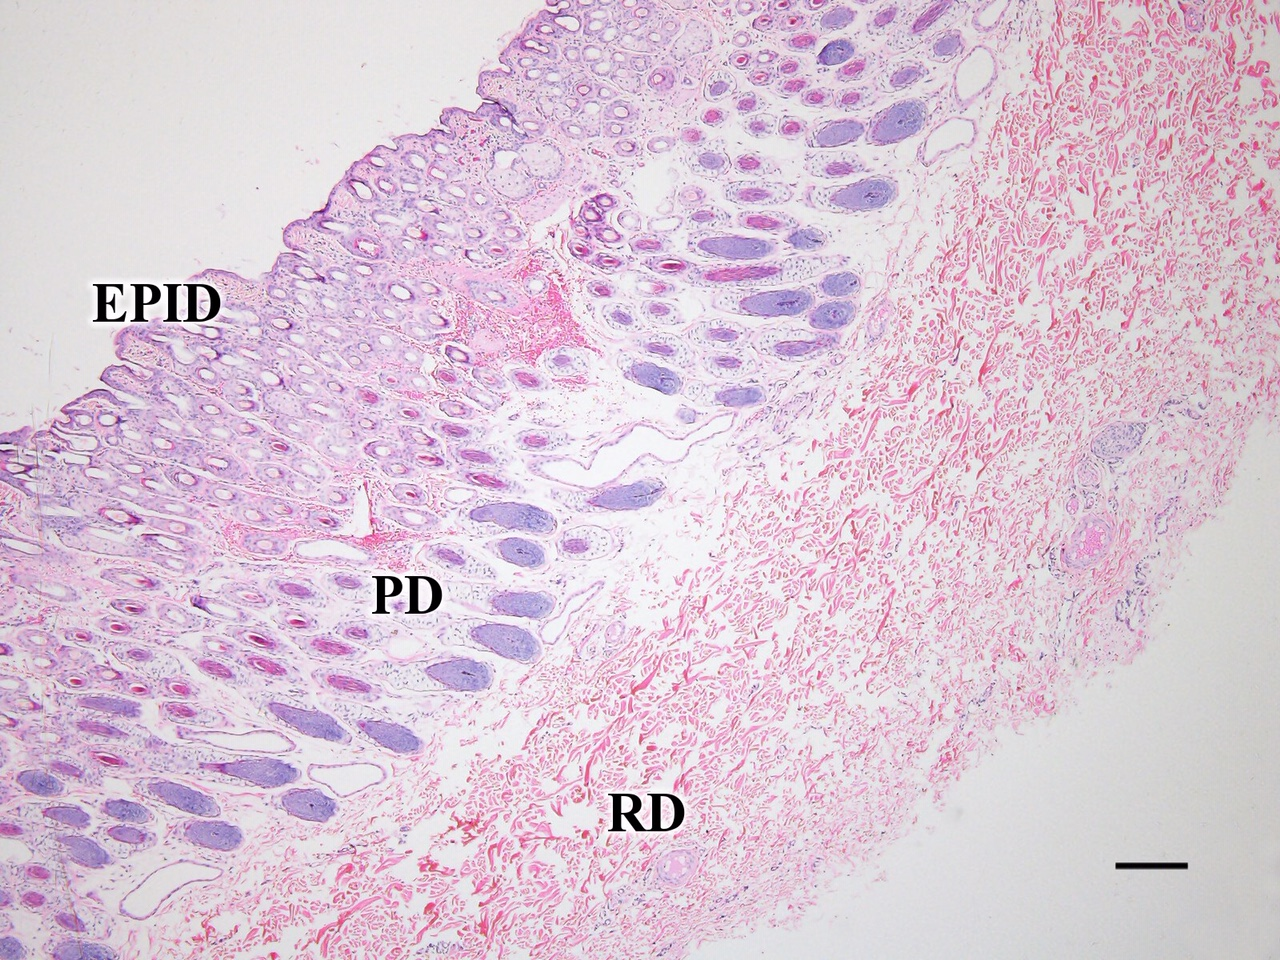
\includegraphics[width=0.7\textwidth]{fig2b.jpg}
  }
  \caption{Vertical sections from a wrinkled (a) and a wrinkle-free (b)  sheep from Trial 2 flock 1 stained with H-E. Skin layers are: {\bf EPID} epidermis, {\bf PD} papillary dermis, and {\bf RD} reticular dermis. Scale bar is 200 $\mu m$ }
\vfill
  \label{fig:trial24xhe}
\end{figure}

%\end{document}

